\documentclass[17pt,
    margin=0.5in,
    innermargin=-4.5in,
    ]{tikzposter}

% Choose size here
\geometry{paperwidth=33.11in,paperheight=46.81in} %A0
% \geometry{paperheight=33.11in,paperwidth=23.4in} %A1
    
\usepackage[utf8]{inputenc}
\usepackage{csquotes}
\usepackage{amsmath}
\usepackage{amsfonts}
\usepackage{amsthm}
\usepackage{amssymb}
\usepackage{mathrsfs}
\usepackage{graphicx}
\usepackage{lipsum}
\usepackage[export]{adjustbox}
%\usepackage{hyperref}
\usepackage{tcolorbox}
\usepackage[font=small,labelfont=bf]{caption} % Required for specifying captions to tables and figures
\usepackage{enumitem}
\usepackage{wrapfig}
%\usepackage[backend=biber,style=numeric]{biblatex}
\usepackage[style=authoryear,backend=biber,
            natbib=true,maxcitenames=1]{biblatex}
\usepackage{glasgow-poster-theme}
\makeatletter
\setlength{\TP@visibletextwidth}{31.0in}
\setlength{ \TP@visibletextheight}{45in}
\makeatother
\usepackage{bm}
\usepackage{bbm}

\addbibresource{references.bib}

% set theme parameters
\tikzposterlatexaffectionproofoff
\usetheme{UniGlasgowTheme}
\usecolorstyle{UniGlasgowStyle}

\usepackage[scaled]{helvet}
\renewcommand\familydefault{\sfdefault} 
\renewcommand{\vec}[1]{\bm{#1}}
\newcommand{\Tr}{\text{Tr}}
\usepackage[T1]{fontenc}

% Adjust trim if title doesn't have two lines
\titlegraphic{\includegraphics[width=0.35\linewidth, trim={0 -2cm 0 0cm}, clip]{figures/logo_glasgow.jpg}}

\title{\parbox{0.8\linewidth}{\textbf{Can the Detection of Roman}\\ \textbf{Roads be Automated with the}\\ \textbf{Application of GeoAI?}}}
\author{Ian Turton\textsuperscript{1}}
\institute{\textsuperscript{1}School of Geographical and Earth Sciences, University of Glasgow, ian.turton@gla.ac.uk}



% begin document
\begin{document}
\maketitle
\centering
\begin{columns}
    \column{0.5}
    \block{Introduction}{
       In the past decade there has been an increased reporting of the use LiDAR data in the discovery of archaeological features in the landscape mainly driven by the increased availability of this type of data as a by-product of flood prevention or forest surveys. Examples from Britain include \citet{gethin_roman_2014} discovering a Roman marching camp and road fragment in North Wales using LiDAR data provided by the Environment Agency, and \citet{small_lost_2016} combines the LiDAR data with other sources to show the route of a Roman road in Southern England. Recently \citet{parcero-oubina_remote_2023} have presented their work on the detection of some previously undiscovered Roman roads in the SW of England using a combination of least cost paths between known Roman occupation locations and then verifying these paths by examining the recently released Environment Agency LiDAR data.

        However, in all of these cases the interpretation and discovery was carried out by a trained archaeologist looking at the LiDAR data set (in a variety of representations) and often by combining it with other information, including the known location of other roman artefacts. There is now 1m resolution LiDAR data available for the much of Great Britain and in many places 50cm resolution data is available freely. This is a data rich problem that is ripe for the introduction of machine learning technology (ML) to winnow the grain from the chaff. \citet{abriha_strategies_2023} look at the use of AI technologies to the discovery of buildings from remote sensed imagery. \citet{albrecht_learning_2019} present the development of a artificial neural network based workflow to detect archaeological features in large LiDAR data.
    }


  \block{Area of Study}{
    \begin{center}
        \includegraphics[width=0.7\linewidth]{figures/scotland.png}
        \captionof{figure}{Known and Postulated Roman Roads in Scotland, after \citet{hanson_roman_2019}}\label{fig:scotland}
    \end{center}
        
   The region for the study (see figure~\ref{figure1}) covers an area between Hadrian's Wall (Carlisle to Newcastle upon Tyne) and the Antonine Wall (Glasgow to Bo'ness). These two walls mark the northern border of the Roman empire in 142CE and 122CE, and there are signs that the Roman engineers planned to proceed further north \citep{margary_roman_1973} with a road extending towards Perth, which is thought to have been the planned basis of a road network in the Highlands of Scotland. There were two main roads, which were constructed before either of the walls were built, a western road from Carlisle across the borders to Edinburgh, and an eastern one (Dere Street) from Corbridge to Dalkeith on the outskirts of Edinburgh \citep{margary_roman_1973}. There were certainly other roads that joined these two main routes to areas of occupation, however the actual route of many of these roads remains unknown (see figure~\ref{fig:scotland}).
    }
    \block{Data Sets}{
        \begin{center}
            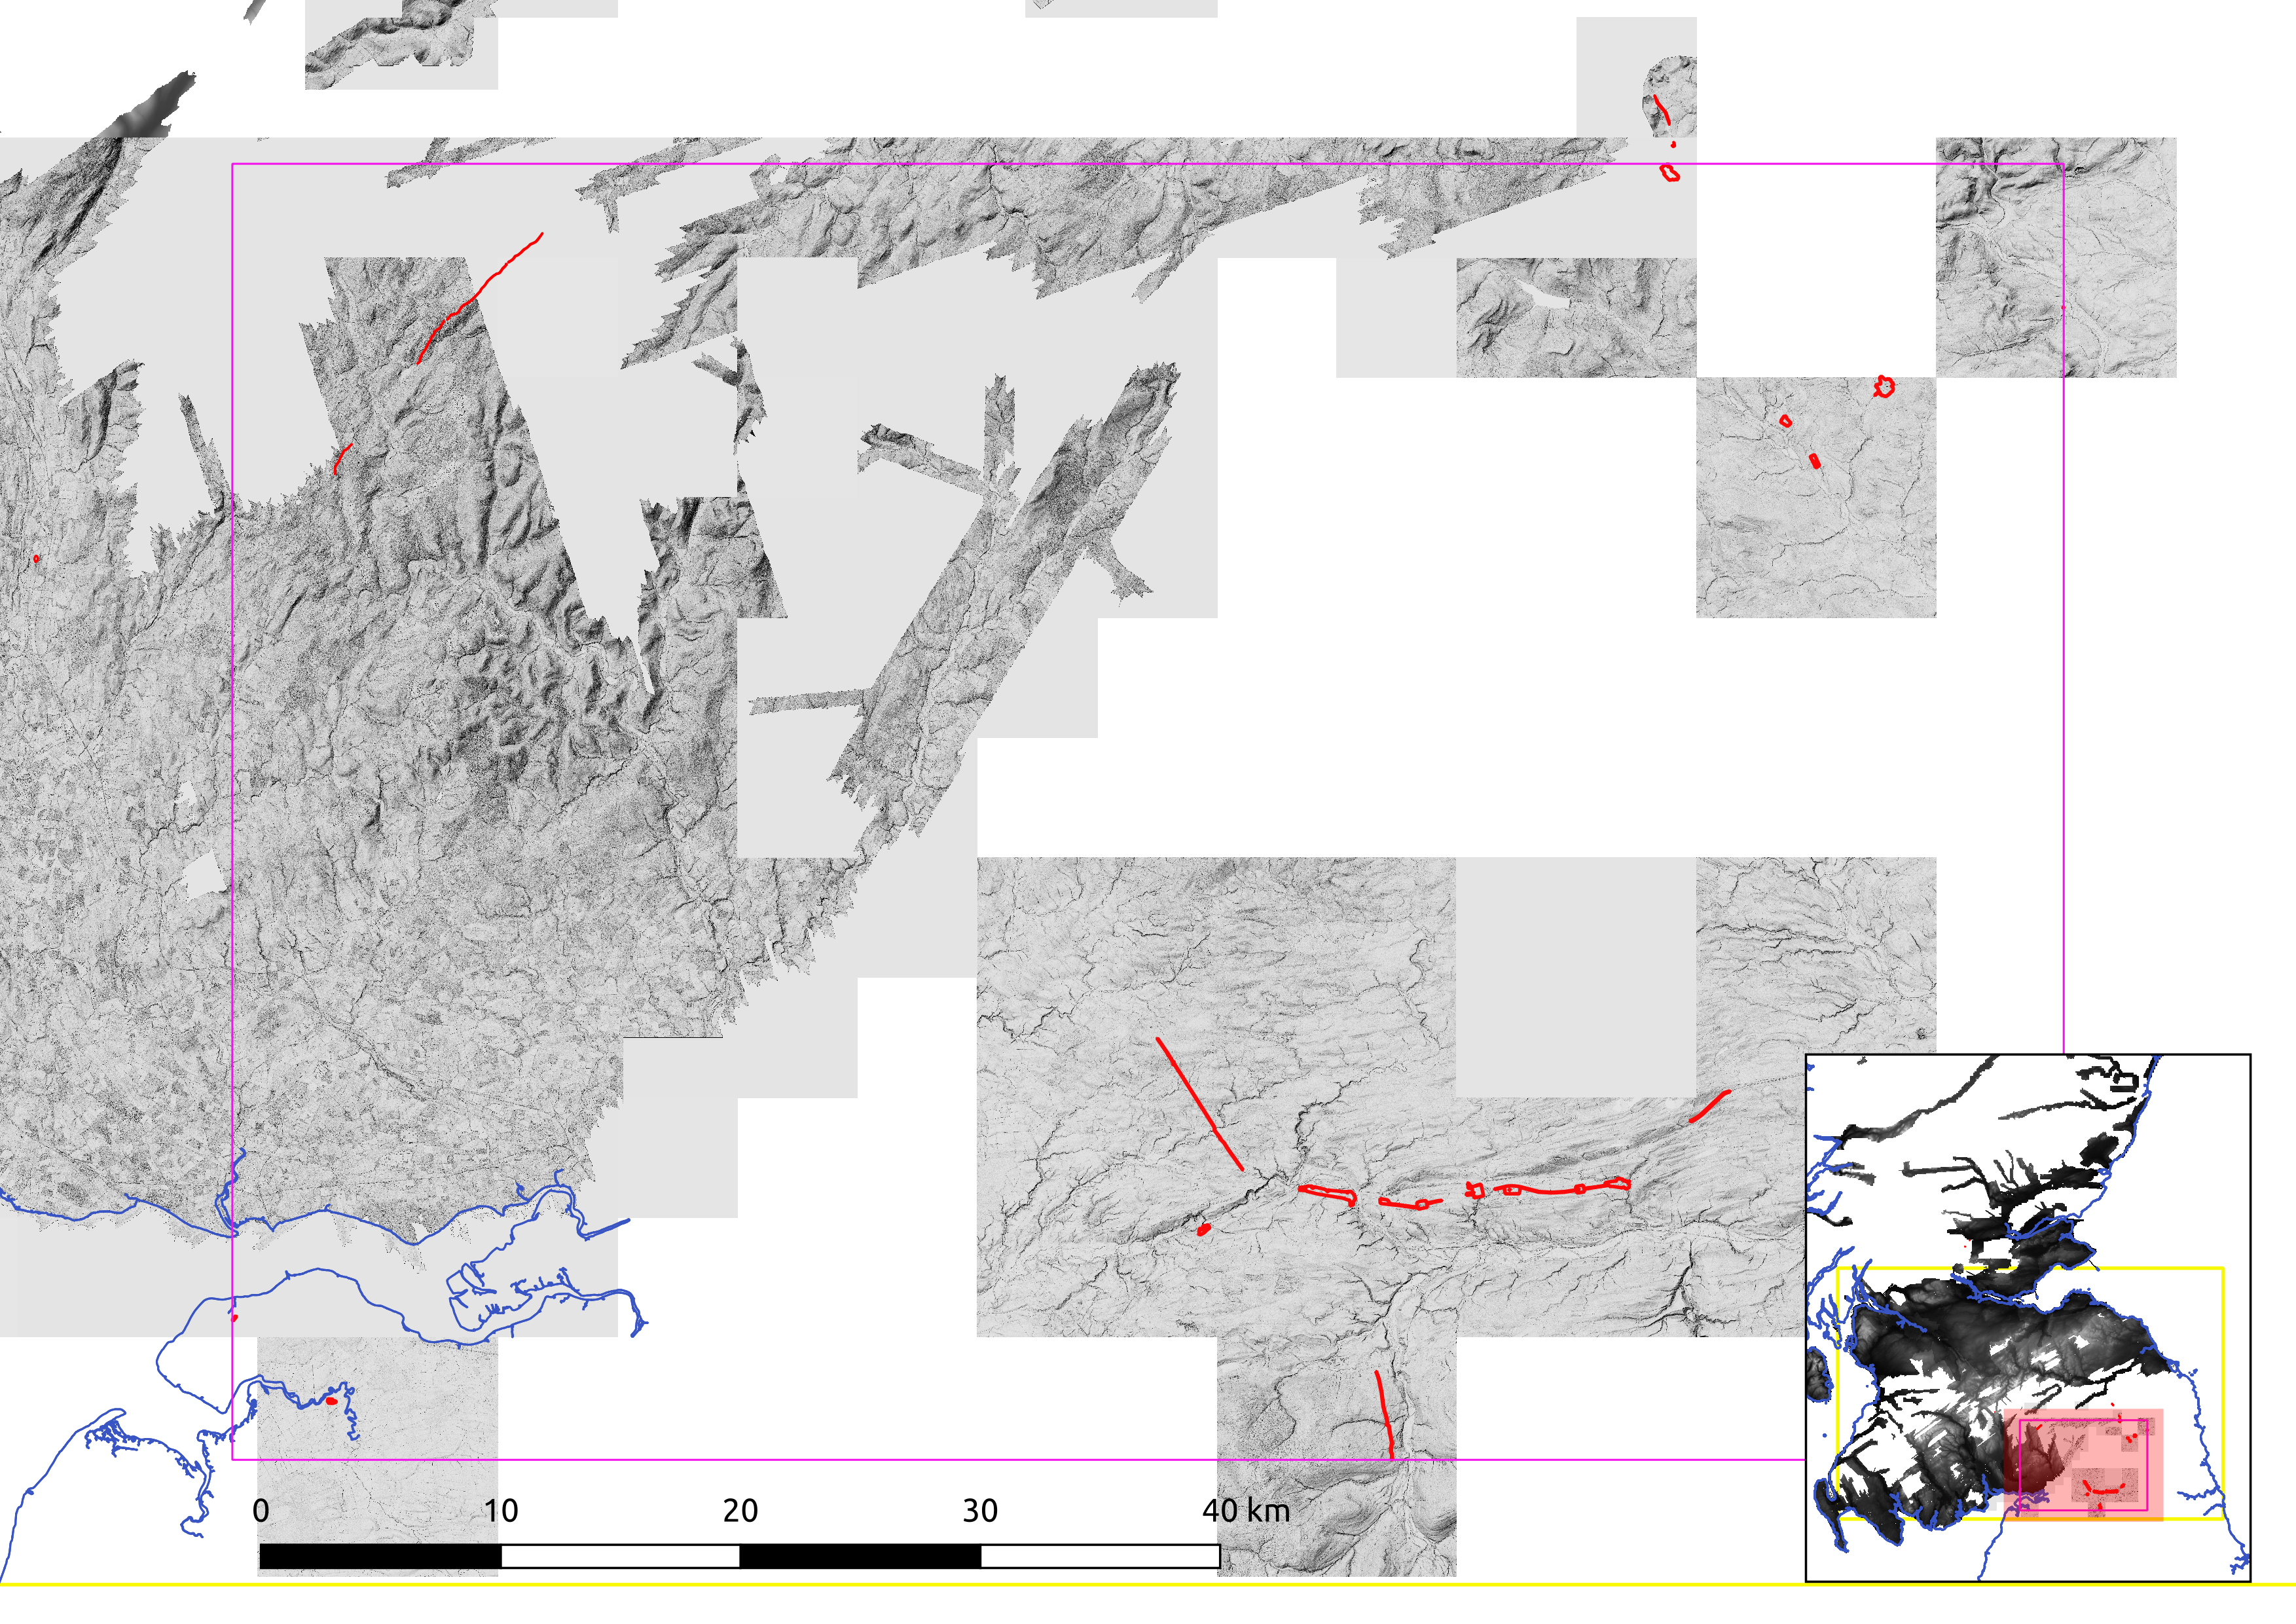
\includegraphics[width=0.7\linewidth]{figures/data_location.png}
            \captionof{figure}{Study region and training data area, showing available LiDAR data and known road locations (in red).}\label{figure1}
        \end{center}
        
       Data used in this study consists of LiDAR data at a horizontal resolution of 50 and 100cm, collected by the English Environment agency (via Digimap) and the Scottish Environment Protection Agency (SEPA). Collecting all the SEPA data was easy as it was available as an S3 bucket in \texttt{tif} format, however the English data could only be collected by 10km grid square and required substantial work to select, download and unpack before reprocessing into a form suitable for GIS use.    
    }
 \block{Methodology}{

    The study planned to convert the LiDAR data to Relief Visualisation Toolbox to produce a visualisation for archaeological topography view as described by \citep{kokalj_why_2019}. The combination of 1.) sky-view factor which provides illumination related to how much of the sky is visible that is limited by relief \citep{zaksek_sky-view_2011}, 2.) the positive openness which highlights the high and low points of the terrain \citep{doneus_openness_2013}, and 3.) a normal hill shading algorithm. The Relief Visualisation Toolbox was unable to handle the size of dataset being considered, requiring tiling the data in to small (500m x 500m) tiles to process. Otherwise, the results were much improved for the detection of features (see figure~\ref{fig:data}).
}

    \column{0.5}

 \block{Methodology continued}{
   
    \begin{center}
            \includegraphics[width=0.6\linewidth]{figures/data_comp.png}
            \captionof{figure}{A comparison of 3 data types: a. 1m resolution DTM, b. visualisation for archaeological topography, c. 25cm aerial imagery}\label{fig:data}
        \end{center}

    \citet{bonhage_modified_2021}, \citet{altaweel_automated_2022}, and \citet{fiorucci_deep_2022} all propose the use of a Mask R-CNN Model which is designed to identify and locate multiple objects in images and generate a segmentation mask for each object found.  The machine learning aspects of the project are made using the \texttt{TorchGeo} package \citep{stewart_torchgeo_2022} which adds many of the needed features needed to handle common spatial data to the \texttt{PyTorch} library \citep{facebook_pytorchpytorch_2024}.   \texttt{PyTorch} is used widely in machine learning tasks, including segmenting images and videos, in many cases a pre-trained model can be fine tuned to work in a new segmentation task. However image processing, generally, have large quantities of high quality training data without missing data or varying resolutions. In geography the images tend to be much larger but often very sparse once missing data is considered. While \texttt{TorchGeo} is designed to take the size of geographic data sets into account, and allows the use of projections and real world units in scaling, it is very much orientated to working with satellite data sets that cover the entire region of study. It is also in it's early stages of development and there are still bugs to be worked around and significant documentation shortages. 

    All machine learning tools depend on a large quantity of data labelled with the expected solution. This study planned to make use of the known scheduled monuments to label where existing known Roman roads could be found, unfortunately the number of known and scheduled roads is too small to provide a sufficient training data set. \citet{bonhage_modified_2021} made use of random reorientation of known sites to provide more variety of training data, but they were working with circular targets and reorientating linear features like roads seems unlikely to help. This lack of targets lead the models developed to fail to detect any features in the training data. 
    }
    \block{Conclusions and Future Work}{
       As currently implemented it appears that \texttt{TorchGeo} is not yet capable of the processing of large, sparse datasets for the detection of archaeological features. Nor, currently, are the commonly used archaeological processing tools ready for use with region geographic datasets, forcing the use of smaller, carefully selected regions of interest. 

       In future work it is hoped to process text from the GB1900 project \citep{university_of_portsmouth_vision_2023} which crowd sourced the text of \textbf{all} the place names and other text on the Second Edition County Series six-inch-to-one-mile maps covering the whole of Great Britain, published by the Ordnance Survey between 1888 and 1914. By finding references to roman artifacts in those maps it may be possible to extend the solution layer which would increase the proportion of training data with a known road present. 

       It is also planned to include aerial imagery in the machine learning process, however due to the difficulty in downloading sufficient imagery one grid square at a time, it is planned to extend the functionality of \texttt{TorchGeo} to be able to process data from a Web Map Server (WMS) layer, this work is progressing well (see \texttt{https://github.com\-/micro\-soft/torchgeo/pull/1965} for details). 


    }
    
    \block{References}{\small
                \begin{center}
                   \mbox{}\vspace{-1\baselineskip}
    \printbibliography[heading=none] 
        \end{center}
        }

    \block{Acknowledgements}{The author acknowledges the support from the UK Research and Innovation Future Leaders Fellowships ``Missing Data as Useful Data'', grant number MR/Y011856/1, ``Indicative Data: Extracting 3D Models of Cities from Unavailability and Degradation of Global Navigation Satellite Systems (GNSS)'', grant number MR/S01795X/2, and the Alan Turing Institute-DSO partnership project on ``Multi-Lingual and Multi-Modal Location Information Extraction''}

\end{columns}
\end{document}